\documentclass[aspectratio=169,11pt]{beamer}

\usepackage[T1]{fontenc}
\usepackage{lmodern}
\usepackage{amsmath}
\usepackage{tikz}
\usetikzlibrary{arrows.meta,positioning,shapes.geometric}

\definecolor{ink}{HTML}{102A43}
\definecolor{blue}{HTML}{2F80ED}
\definecolor{teal}{HTML}{00897B}
\definecolor{amber}{HTML}{F2C94C}
\definecolor{red}{HTML}{C94C4C}
\definecolor{mist}{HTML}{F4F7FA}
\definecolor{line}{HTML}{B7C4D1}

\setbeamercolor{normal text}{fg=ink,bg=white}
\setbeamercolor{frametitle}{fg=ink,bg=white}
\setbeamerfont{frametitle}{size=\fontsize{25}{28}\selectfont,series=\bfseries}
\setbeamersize{text margin left=0.60cm,text margin right=0.60cm}
\setbeamertemplate{navigation symbols}{}
\setbeamertemplate{frametitle}{\vspace{0.18cm}\hspace{0.45cm}\insertframetitle\par}
\setbeamertemplate{footline}{%
  \hspace{0.45cm}\color{line}\rule{15.1cm}{0.35pt}\par
  \vspace{0.05cm}\hspace{0.45cm}\scriptsize\color{ink}
  \insertshorttitle\hfill\insertframenumber\hspace{0.45cm}\vspace{0.14cm}}
\title[Current BB144 OSD-0 RTL]{Current BB144 OSD-0 RTL}

\tikzset{
  flow/.style={-Latex,very thick,draw=ink},
  box/.style={draw=line,very thick,rounded corners=2pt,fill=mist,
              align=center,minimum height=1.05cm,font=\fontsize{13}{15}\selectfont},
  bp/.style={box,draw=blue,fill=blue!8},
  osd/.style={box,draw=teal,fill=teal!8},
  result/.style={box,draw=teal,fill=teal!12},
  decision/.style={diamond,aspect=2.0,draw=ink,very thick,fill=white,
                   align=center,font=\fontsize{12}{14}\selectfont},
  note/.style={font=\fontsize{12}{14}\selectfont,align=left},
  label/.style={font=\fontsize{10.5}{12}\selectfont,fill=white,inner sep=1.5pt},
}

\begin{document}

\begin{frame}[t]{OSD-0 begins where BP stops}
  \vspace{-0.18cm}
  {\fontsize{13.5}{16}\selectfont
   BB144 Z-check sector: $m=936$, $n=8784$, with 7-bit final BP marginals $L_j$.}

  \vspace{0.16cm}
  \makebox[\textwidth][c]{\resizebox{0.97\textwidth}{!}{%
  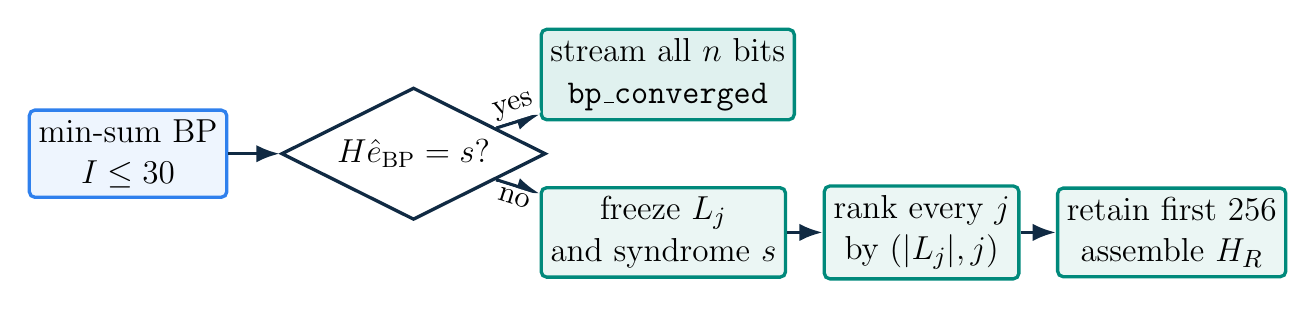
\begin{tikzpicture}
    \node[bp,minimum width=2.0cm] (bp) {min-sum BP\\$I\leq30$};
    \node[decision,minimum width=2.35cm,right=0.65cm of bp] (check)
      {$H\hat e_{\rm BP}=s$?};
    \node[result,minimum width=2.45cm,above right=-0.02cm and 0.75cm of check] (done)
      {stream all $n$ bits\\\texttt{bp\_converged}};
    \node[osd,minimum width=2.30cm,below right=-0.02cm and 0.75cm of check] (freeze)
      {freeze $L_j$\\and syndrome $s$};
    \node[osd,minimum width=2.35cm,right=0.45cm of freeze] (sort)
      {rank every $j$\\by $(|L_j|,j)$};
    \node[osd,minimum width=2.60cm,right=0.45cm of sort] (reduce)
      {retain first 256\\assemble $H_R$};
    \draw[flow] (bp) -- (check);
    \draw[flow] (check) -- node[label,above,sloped]{yes} (done);
    \draw[flow] (check) -- node[label,below,sloped]{no} (freeze);
    \draw[flow] (freeze) -- (sort);
    \draw[flow] (sort) -- (reduce);
  \end{tikzpicture}}}

  \vspace{0.10cm}
  \begin{columns}[T,onlytextwidth]
    \begin{column}{0.30\textwidth}
      {\color{blue}\bfseries\fontsize{15}{17}\selectfont Sparse source}\par\smallskip
      {\fontsize{11.5}{13.5}\selectfont
       \texttt{col\_ones[j]} lists touched checks; the full
       $936\times8784$ matrix is not runtime state.}
    \end{column}
    \begin{column}{0.34\textwidth}
      {\color{teal}\bfseries\fontsize{15}{17}\selectfont Assemble on drain}\par\smallskip
      {\fontsize{11.5}{13.5}\selectfont
       Ranked $j$ enters slot $r$; set $H_R[i,r]=1$ for every
       $i\in\texttt{col\_ones[j]}$.}
    \end{column}
    \begin{column}{0.30\textwidth}
      {\color{teal}\bfseries\fontsize{15}{17}\selectfont Stored state}\par\smallskip
      {\fontsize{11.5}{13.5}\selectfont
       $H_R\in\mathbb F_2^{936\times256}$: 239,616 bits plus
       256 original indices.}
    \end{column}
  \end{columns}

  \vspace{0.05cm}
  {\color{red}\fontsize{10.5}{12.5}\selectfont
   \textbf{Current policy:} all 8784 columns drain; retain the first
   $R_{\max}=256$ (no $|L|$ filter).}
\end{frame}

\begin{frame}[t]{One ranking, three solver widths}
  \vspace{-0.18cm}
  {\fontsize{13.5}{16}\selectfont
   The $64\to128\to256$ retries reuse the same order and $H_R$: no BP rerun, no re-sort.}

  \vspace{0.14cm}
  \makebox[\textwidth][c]{\resizebox{0.98\textwidth}{!}{%
  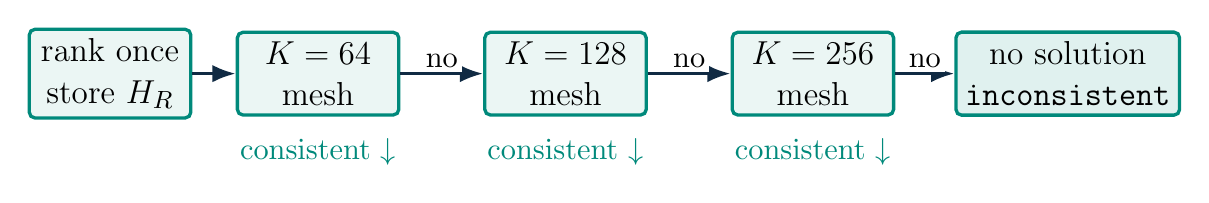
\begin{tikzpicture}
    \node[osd,minimum width=2.05cm] (rank) {rank once\\store $H_R$};
    \node[osd,minimum width=2.05cm,right=0.55cm of rank] (k64)
      {$K=64$\\mesh};
    \node[osd,minimum width=2.05cm,right=1.05cm of k64] (k128)
      {$K=128$\\mesh};
    \node[osd,minimum width=2.05cm,right=1.05cm of k128] (k256)
      {$K=256$\\mesh};
    \node[result,minimum width=2.35cm,right=0.75cm of k256] (fail)
      {no solution\\\texttt{inconsistent}};
    \draw[flow] (rank) -- (k64);
    \draw[flow] (k64) -- node[label,above]{no} (k128);
    \draw[flow] (k128) -- node[label,above]{no} (k256);
    \draw[flow] (k256) -- node[label,above]{no} (fail);
    \node[font=\fontsize{11}{13}\selectfont,text=teal,below=0.15cm of k64]
      {consistent $\downarrow$};
    \node[font=\fontsize{11}{13}\selectfont,text=teal,below=0.15cm of k128]
      {consistent $\downarrow$};
    \node[font=\fontsize{11}{13}\selectfont,text=teal,below=0.15cm of k256]
      {consistent $\downarrow$};
  \end{tikzpicture}}}

  \vspace{0.20cm}
  \begin{beamercolorbox}[wd=\textwidth,sep=0.16cm,center,rounded=true]{block body}
    {\color{teal}\fontsize{13}{15}\selectfont
     Stream $(\texttt{selectedIndex}[r],x_r)$; every unselected correction bit is zero.}
  \end{beamercolorbox}

  \vspace{0.22cm}
  \begin{columns}[T,onlytextwidth]
    \begin{column}{0.47\textwidth}
      {\color{blue}\bfseries\fontsize{15}{17}\selectfont Active-row stream}\par\smallskip
      {\fontsize{11.5}{13.5}\selectfont
       Solve $H_R[:,0{:}K]x_K=s$. Stream only rows with nonzero
       coefficients or $s_i=1$; call their count $m'_K$.}
    \end{column}
    \begin{column}{0.47\textwidth}
      {\color{teal}\bfseries\fontsize{15}{17}\selectfont Cycle and area consequences}\par\smallskip
      {\fontsize{11.5}{13.5}\selectfont
       Sort: 17,568 clocks. Attempt $K$: $m'_K+3K+1$;
       solved output: $K$. All three meshes exist, but only one is active.}
    \end{column}
  \end{columns}

\end{frame}

\end{document}
